\documentclass[a4paper]{profusion}

\usepackage{verbatim}
\usepackage{graphicx}
%\usepackage{ctable}
%\usepackage{longtable}
%\usepackage{rotating}
%\usepackage{makecell}

%\bibliographystyle{plain}

\def\fboxsep{5pt}
  \newenvironment{myboxenv}[1]
  {
    \begin{flushright}
      \begin{boxedminipage}{0.9\textwidth}
        \textbf{%% \sffamily
          \large #1:}

        \hspace{-5pt}\rule{0.3\textwidth}{0.5pt}
        \begin{center}
          \begin{minipage}{0.95\textwidth}

            \small%% \slshape
         }
          {
          \end{minipage}
        \end{center}
      \end{boxedminipage}
    \end{flushright}
 }

  \newenvironment{note}
  {
    \begin{myboxenv}{
        
\includegraphics[scale=0.4]{images/note.pdf}
        Note}
   }
    {
    \end{myboxenv}
 }

  \newenvironment{warning}
  {
    \begin{myboxenv}{
        
\includegraphics[scale=0.5]{images/attention.pdf}
        Warning}
   }
    {
    \end{myboxenv}
 }

  \newenvironment{important}
  {
    \begin{myboxenv}{
        
\includegraphics[scale=0.5]{images/important.pdf}
        Important}
   }
    {
    \end{myboxenv}
 }


\title{The Enlightenment Foundation Libraries\\
  \normalsize{A Big Picture}}

\ProFUSIONMail{glima@profusion.mobi}
\author{Gustavo Lima Chaves}

\begin{document}

\maketitle
\tableofcontents

\section{Introduction}

The Enlightenment Foundation Libraries, or simply EFL, are a set of
software libraries that grew up to support the Enlightenment desktop
shell and the applications using its same technology. They have
historically been built with high optimizations in mind, targeted not
only to desktop computers, but also to low-end devices.

In this document a big picture of this set of libraries and their
correlation is going to be presented, so that software developers
totally unaware of them can rapidly learn the basics and start using
the EFL.

\section{The e-libs' basics}

EFL developers tend to name their libraries with something beginning
with the letter ``e''. In this document we'll talk about the following
ones: evas, ecore, eet, edje and elementary. This section gives a
brief overview of these 5 libraries, before we get a little deeper
inside each of them.

\subsection{Evas}

Evas is a fundamental piece in the set -- it is the \emph{canvas}
library, which manages the graphical objects one wishes to exhibit and
deals directly with back-end engines closer to the hardware display
drivers. Of course, it abstracts any need to know the characteristics
of your display system or which graphics calls are in fact used to
draw on the screen.

Unlike other canvas objects (or widgets) provided by most of the
graphical user interface libraries (GUIs) out there, evas is specially
powerful. It is a \emph{stateful} canvas in that it keeps track of
which objects must and mustn't be rendered on screen. It does the
so-called \emph{retained mode drawing}, in opposition to the
\emph{immediate mode drawing}. The programmer has no need of dealing
with objects repainting or keeping their state. Evas optimizes the
rendering pipeline to minimize the effort in redrawing changes made to
the canvas and so takes this work out of the programmer's hand, saving
a lot of time and energy.

Evas has no notion of \emph{time} and \emph{animations}, things that
are made available to the programmer by combining it with other
e-libs.

This library is intended to deal with \emph{raster graphics}. Its
powerful (super and sub-sampled) smooth-scaling algorithms guarantee
fancy graphics even when different sizes of an image are needed. It
ships with loaders of gif, jpeg, png, tiff and xpm image files. It can
save them back, possibly after painting something on top of them or
applying one of its transformations, into jpeg, png and tiff formats.
Evas can also draw anti-aliased text, alpha-blend objects and much
more.

Finally, evas supports \emph{many} different back-end engines. This,
paired with its highly optimized drawing methods, permit that the
library can be used on a large variety of systems, including low-end
embedded devices.

\subsection{Ecore}

Ecore is a like a ``swiss knife'' library for the e-world. One can
resume its purpose as a library that gives developers higher level
interfaces for low-level stuff (and also convenience functions). It
also provides, for example, facilities evas was not meant to have,
like event handling and timers.  Moreover, ecore is the library which
provides the \emph{main loop} for the applications using EFL
technology (though one is not restricted to it).

This library also provides wrappers on top of evas, simplifying a bit
the chain of functions needed to instantiate and manage a
canvas. Other facilities found on ecore are sockets abstraction, IPC,
configuration handling, etc.

\subsection{Edje}

Edje is a special library even between the EFL ones. It is a powerful
and pioneer \emph{layout engine} and graphical design tool based on
evas.

\begin{note}
On the words of its creator:\\

``Edje is an attempt to find a middle ground between theming and
programming without turning the theme itself into just yet another
program.'' -- Carsten Haitzler (The Rasterman)
\end{note}

It provides an abstraction layer between the application code and its
interface, besides allowing for extremely flexible dynamic layouts and
animations. More precisely, it interprets files compiled from a
declarative language which allows one to describe a graphical user
interface without writing a single line of the working programming
language's code. In other words, your application is split into two
parts: a graphical part, which knows nothing about (functionality)
code and the functionality, which knows nothing about its GUI.

This brings more freedom to both programmers and interface designers.
Once a contract between the program's back-end and its interface is
established (which is done mainly in terms of signals, to be better
explained further), developers can easily change the back-end's
functionality independently of the GUI and vice-versa.

This concept, for ages already supported by the EFL, has more and more
drawn  people's  attention  and  has  recently  been  called
\emph{declarative user interfaces}.

In terms of implementation, one can say that edje is a \emph{state
 machine}. When declaring an interface visual element, the designer
describes one or more \emph{states} that element can be at. These
states can differ in many parameters, for example:
\begin{itemize}
\item object's position and size,
\item object's color and opacity,
\item object's visibility,
\item object's response to input events, etc.
\end{itemize}

Naturally, edje holds, internally, a geometry state machine and a
state graph of what is visible (or not), where, at what size, with
what colors, etc.

Speaking of input events, a great feature of this library is that one
can specify, besides element states, actions triggered by different
input actions and \emph{transitions} to optionally occur after
them. Input events may be mouse ones (hover, click, etc), signals from
the application's back-end, etc. There are some built-in transition
timelines (being their total time a parameter) which take one object
from origin to target states.  Examples of them are: linear,
accelerated and sinusoidal transitions (see section \ref{sec:progs}).

Edje allows for \emph{real} theming capabilities: applications can have
interfaces \emph{completely} different one from another and with
different behavior, too. One describes an interface in the form of an
\emph{edje data collection} (EDC), which is a plain text file with
simple syntax to describe the interface's visual elements and their
behavior. This is so that the visual elements' descriptions, along
with their image sources, when applicable, and the fonts used by text
elements are all packaged together into a \emph{single} file. This
way, whole themes of interfaces can be shipped around with great
facility.

A designer has the ability to animate, layout and control the
look-and-feel of any program using edje as its basic GUI
constructor. Naturally, if one needs a more specific element behavior
or look-and-feel, new visual objects can be built from scratch, with
the help of a developer, who will be using evas directly.

\subsection{Eet}

Eet is a tiny library whose API lets the programmer write an arbitrary
set of chunks of data to a file (optionally compressing them, very
much like a zip file) while allowing fast random-access reading of
this file later on. EET files, as they are called, are perfect for
storing data that are written once (or rarely) and read many times,
especially when the programmer wants to avoid the necessity of reading
all the stored data at once.

Two common use cases for this library are:
\begin{itemize}
\item storing configuration data and
\item \emph{storing themes}.
\end{itemize}

EDC files are processed by a binary distributed with edje, \emph{the
 edje compiler}, which packs the interface's description and data
altogether in the form of an EET file. People have historically named
these interface files with the \texttt{.edj} extension.  For now on,
we'll refer to these specific EET files as \emph{EDJ files}.

Besides we cite just these two use cases, many more exist for eet. One
can store \emph{arbitrary} data chunks at EET files. There are
developers storing javascript scripts in it, for example.

\subsection{Elementary}

Elementary is a basic widget set library built on top of other e-libs
(mainly evas, ecore, and edje) that is easy to use. It was created,
originally, aiming development for mobile touch-screen devices.

This is just one of the ways, while using EFL technologies, of
creating visual elements besides using pure edje (or even pure
evas). Elementary provides many built-in widgets to the programmer,
like:

\begin{itemize}
\item icons,
\item buttons,
\item scroll bars,
\item labels, etc.
\end{itemize}
All these widgets are themeable, of course.

Elementary also provides higher level abstractions and control. For
example, the library enables operations which affect the whole
application's window, with functions to lower it, raise it, maximize
it, rotate it and the like. Also, with elementary the user may set the
``finger size'' (finger-clickable widgets' sizes) intended for use on
a touchscreen application, affecting all the widgets with finger
interaction.

\section{Ecore-evas}
Ecore-evas is one of ecore's modules you'll certainly want to use.  It
is a set of convenience functions around evas, which save you from
lots of low level interaction with drawing engines, canvas update and
maintenance calls and the like.

All graphic engines evas supports have respective high level
functions, found at ecore-evas, to:

\begin{itemize}
\item instantiate a canvas, bound to that back-end engine, with a
  given geometry, and
\item retrieve the application's window, if the graphic back-end
  implements windows.
\end{itemize}

Besides that, ecore-evas gives you generic canvas manipulation
functions, regardless of the engine being used. For example, you can:
\begin{itemize}
\item set callback functions on canvas events like resize, move,
  gain/loss of focus,
\item perform actions on the canvas like move, resize, set the title,
  set fullscreen mode, etc.
\end{itemize}

Ecore-evas, finally, integrates the calls of canvas updating
(re-calculation of object states and re-renderization) into ecore's
main loop, so that the user mustn't deal with it.

\section{Evas and its \emph{objects}}

The basic evas object unit one is going to interact with is the
\texttt{Evas\_Object}. This is a C opaque type which represents a
generic visual element evas handles and draws. \texttt{Evas\_Objects}
have, naturally, a \emph{type} associated with them, so that
specialization is possible.

Evas has a set of built-in object types\footnote{Actually there is an
  object for multi-line text entries, too.}:
\begin{itemize}
\item rectangle,
\item line,
\item polygon,
\item text,
\item image.
\end{itemize}

The ones which are most used are rectangles, text and images. In fact,
with these ones one can create 2D interfaces of arbitrary complexity
and EFL makes it easy!

%% \textcolor{red}{TODO: More on the base types here? The common API?}

However, people are not at all limited to these objects. Evas lets you
build objects of arbitrary complexity with the concept of \emph{smart
  objects} (SOs).  Beginning from a basic \texttt{Evas\_Object}, one
can specify a basic interface to this new object (function pointers
like \texttt{add}, \texttt{del}, \texttt{move}, \texttt{resize},
\texttt{show}, etc.) that form the common set of evas interaction
routines over its objects.  More importantly, SOs can have other
objects as their \emph{children}. Smart objects' behavior can be so
that the outer operations executed on them reflect on a custom manner
over each of the child objects.

Besides having to be built a little differently than simple built-in
objects, smart objects end up with the same opaque type for use by the
programmer: \texttt{Evas\_Object}. When building a widget set,
programmers have this instantiation steps hidden away from the API
users, so that the creation of evas smart objects end up as simple as
the base ones (just one function call).

Evas comes with three built-in smart object types, whose descriptions
follow.

%\subsection{Box Objects}
\begin{description}

\item[Box Objects] A box container is a smart object intended to have
  child elements, displaying them at \emph{sequential order}. It can
  layout the child elements in various different ways, though. It has,
  in its API, functions to set the desired layout, with the
  possibility of using layouting functions other than the built-in
  ones.

%\subsection{Table Objects}
\item[Table Objects] A table container is a smart object also intended
  to have child elements, displaying them in a \emph{table} (or grid)
  form.  Again, one can choose between some built-in layouts, but
  there is no support for custom layouts for these objects.

%\subsection{Edje Objects}

\item[Edje Objects] This is how, at programming level, edje and evas
  fit together. Visual elements whose appearance and behavior are
  controlled by edje are nothing more than evas smart objects. Edje
  encapsulates all the instantiation steps of these objects inside
  itself. We'll see, further, that after instantiation, an edje
  (smart) object must have an EDJ file set to it. This operation also
  requires that a \emph{group}\footnote{``Groups'', as will be
    explained further, are declaration blocks of edje data collections
    which pack together visual elements, or ``parts''.}, declared
  inside that EDJ, is associated with this object. This group tells
  about all of the child elements this edje object has. These can be
  any evas object, including the smart ones (note the recursive
  aggregation possibilities, here).
\end{description}

Elementary's widgets, as one might expect, are also evas smart
objects.

Finally, any \texttt{Evas\_Object} may have \emph{hint fields}
set. Their objective is to guide the e-libs' functionality in some way
while layouting and displaying that object. These hints may affect,
for example:
\begin{itemize}
\item object sizes (both horizontal and vertically),
\item object alignment inside a container and
\item object padding.
\end{itemize}

Hints are not always enforced (and may be treated just like hints,
then). Actual sizes of an object, for example, are properties separate
from the size hints. The latter will never be used in calculations
which involve the object's sizes.

SOs may implement any custom behavior for the values they get from
these fields. For example, box objects use alignment hints to align
its lines/columns inside its container, padding hints to set the
padding between each individual child, etc. Edje uses size hints to
layout its objects, too. We'll see, further, that edje exposes some of
these hint fields at the EDC language.

\section{Playing Edje with Edje Data Collections}

We shall begin a deeper study of edje concurrently with the
presentation of the language it interacts with. As previously said,
the way one describes, to edje, a graphical user interface is through
a simple declarative language. A text file is written containing
(possibly) several sections, which can describe:
\begin{itemize}
\item the images and fonts to be used in the interface,
\item what visual elements should the interface have and how they
 should be laid out,
\item actions (or ``programs'') to occur when the interface is
 interacted with.
\end{itemize}
Programs can be further supplemented by employing scripting languages,
which   add  some   programability   to  the   interface's
behavior\footnote{This topic will be readdressed later.}.

These text files, which we call edje data collections, are commonly
named with the \texttt{.edc} extension. They are not parsed at this
form at run time, though. They must be previously compiled into a
binary, more succinct form, which includes the binary blobs of the
images, the fonts, etc.  As said before, all the interface's
descriptions and data are packed together in an EET file, which is
customarily named with the \texttt{.edj} extension. EDJ files are the
output of the \texttt{edje\_cc} compiler, whose basic invocation is
something like:

\begin{verbatim}
edje_cc input_file.edc output_file.edj
\end{verbatim}

At run-time, the application loads the EDJ file(s) through edje's API.
Then, edje automatically generates the evas objects necessary to
display the interface.

Because of the great simplicity in having all the interface
information in only one file, changing an EFL-based application's
theme is a mere question of loading it with a different EDJ
file. These interchangeable interface versions must only adhere to the
same ``contract'', that is, the way they communicate with the
software's back-end. For this reason, people in the e-world often call
EDJ files directly with the term \emph{theme}. We are going to use
these terms interchangeably here, too.

The syntax for EDC files follows a simple structure of brace-enclosed
blocks that can contain properties, more blocks, or both. We shall,
now, describe the main building blocks of this language. For each
block, we give an example of use at the beginning of its section.

A thorough description of this language can always be consulted at the
Edje Data Collection Reference web page, found at \url{
  http://docs.enlightenment.org/auto/edje/edcref.html}.

\subsection{Macros}

\texttt{edje\_cc} uses the C pre-processor to expand macros. Then, all
if its macros may be used, like:
\begin{itemize}
\item \texttt{\#define}
\item \texttt{\#include}
\item \texttt{\#ifdef}/\texttt{\#endif}, etc.
\end{itemize}

\subsection{Top-level blocks}

The main top level blocks which can go into an EDC file are the ones
declaring:
\begin{itemize}
\item images,
\item fonts,
\item data (in string form),
\item styles and
\item collections.
\end{itemize}

When declared globally, they are visible throughout the whole edje
data collection. Most of them can be defined at more restricted
scopes, which can be more convenient in some cases.

\subsubsection{Images}

\begin{lstlisting}
images {
    image: "filename1.ext" COMP;
    image: "filename2.ext" LOSSY 99;
}
\end{lstlisting}

The \texttt{images} block is used to list each image file that will be
used in the theme along with its compression method (if any). This
information block, besides the EDC file's top level, can occur inside
lower level blocks, easing the maintenance of the file list when the
theme is split among multiple files\footnote{Remember the
  \texttt{\#include} macro.}.

The general rule to include each image is:

\begin{verbatim}
image: "[path_to_image_file]" [compression_method] [compression_level];
\end{verbatim}

The full path to the directory holding the images can be defined later
with \texttt{edje\_cc}'s ``\texttt{-id}'' option. These image files
must match one of the types evas was compiled with support to.
Usually png and jpeg formats are supported, but it depends on how evas
was compiled.

 The compression methods may be the following:

\begin{description}
\item[\texttt{RAW}] uncompressed,
\item[\texttt{COMP}] lossless compression and
\item[\texttt{LOSSY [0-100]}] lossy compression with quality from 0 to
 100.
\end{description}

\subsubsection{Fonts}

\begin{lstlisting}
fonts {
    font: "file_name1.ext" "font_alias";
    font: "file_name2.ext" "other_font_alias";
}
\end{lstlisting}

The \texttt{fonts} block is used to list each font file with an
\emph{alias} used later in the theme, besides including the font
itself into it. Similarly to the \texttt{images} one, \texttt{fonts}
blocks may be included inside other blocks. The full path to the
directory holding the fonts can be defined later with
\texttt{edje\_cc}'s ``\texttt{-fd}'' option.

Evas (and consequentially edje) can be compiled with fontconfig
support.  When it's done, system fonts may be accessed by name and
style parameters, like in ``\texttt{Sans Serif:style=Bold}''.

\subsubsection{Data}

\begin{lstlisting}
data {
    item: "key" "value";
    file: "other_key" "file_name.ext";
}
\end{lstlisting}

The \texttt{data} block is used to pass arbitrary parameters (in the
form of strings) from the theme to the application.  This can be
useful, for example, in a scenario where the software back-end
programmer had in mind more them one GUI schema, being them discrepant
to the point that visual elements (which translate, in edje, to groups
and parts, as will be further explained) exist in one of them but not
on the other. The themes could signal that in the form of a data
field, and the back-end would them interact with the right visual
parts for each case.

The properties defined for this block have two possible forms:
\begin{description}
\item[\texttt{item: "[key]" "[value]";}] This defines a new data item
  whose value will be the string specified in the \texttt{value}
  field.
\item[\texttt{file: "[key]" "[filename]";}] This defines a new data
  item whose value will be the contents of the specified file formatted
  as a single string of text. Naturally, this property only works with
  plain text files.
\end{description}

This block  may also occur inside  \texttt{group} blocks, thus,
having only that scope.

\subsubsection{Styles}

\begin{lstlisting}
styles {
    style {
        name: "style_name";
        base: "font_size=14 color=#ffffff valign=baseline";
        tag: "br" "  \n";
    }
}
\end{lstlisting}

The  \texttt{styles} block  contains a  list of  one  or more
\texttt{style} blocks, which are used to create \emph{style tags} for
advanced \texttt{TEXTBLOCK} formatting.

\texttt{TEXTBLOCK}s are one type of visual elements native to edje
which, naturally, exhibit text. We'll get back to them further in this
text.

The properties to be filled at a \texttt{style} block are:
\begin{description}
\item[\texttt{name: "[style\_name]";}] The name of this style, to be
  referenced later in the theme.
\item[\texttt{base: "[style\_properties\_string]";}] The default style
  properties that will be applied to the complete text. The syntax of
  this string is going to be presented further.

  %% \textcolor{red}{TODO:  define the syntax here? Further?}

\item[\texttt{tag: "[tag\_name]" "[style\_properties\_string]";}]
  Style to be applied only to text between tags in the form
  \texttt{<tag\_name>}, \texttt{</tag\_name>}.
\end{description}

The \texttt{styles} block can also occur inside lower level blocks.

\subsubsection{Collections}

\begin{lstlisting}
collections {
    images { /*...*/ }
    fonts { /*...*/ }
    styles { /*...*/ }

    group { /*...*/ }
}
\end{lstlisting}

The \texttt{collections} block is used to group \texttt{images},
\texttt{fonts}, \texttt{styles} and \texttt{group} blocks altogether,
defining a ``groups scope''. Additional \texttt{collections} blocks do
not prevent overriding of groups with equal names, though.

\subsection{Packing cohesive visual elements together: the \texttt{group}
 block}

%% \textcolor{red}{TODO: does a programs block make sense here?}
    %% programs { /*...*/ }

\begin{lstlisting}
group {
    name: "name_used_by_the_application";
    alias: "another_name";
    min: 100 200;
    max: 100 9999;

    data { /*...*/ }
    script { /*...*/ }
    images { /*...*/ }
    fonts { /*...*/ }
    styles { /*...*/ }

    parts { /*...*/ }
}
\end{lstlisting}

A \texttt{group}, broadly, defines the contents of an edje smart
object.  An edje SO, which is a very elaborate kind of SO, may
correspond to a GUI's whole screen, a widget, or simply a part of a
screen.  The child elements of an edje object are declared as EDC
\texttt{part}s.  All of evas' built-in objects are supported,
obviously, and so are smart objects. Actually, a part may be another
group itself, reflecting on edje data collections the recursive object
aggregation possibilities evas gives us.

Being an edje object a really smart one, in what it has edje's state
machine supporting it, one can declare, at EDCs, \emph{programs}. As
said before, these are actions occurring after user (or back-end)
interaction with the visual objects composing the edje SO. The
\texttt{programs} block is presented at section \ref{sec:progs}, while
the \texttt{script} one is explained at section \ref{sec:scripts}.

Some properties one can define at a \texttt{group} are:

\begin{description}
\item[\texttt{name: "[group\_name]";}] The name that will be used by
  the application to load the resulting edje object or by the EDC
  writer himself, when nesting groups.  If more than one group,
  \emph{with the same name}, exist in an EDC file, the last one's
  definition is going to override the others'.

\item[\texttt{alias: "[additional\_group\_name]";}] Additional name to
  serve as this group's identifier. Defining multiple aliases is
  supported.

\item[\texttt{min: "[width]" "[height]";}] The \emph{size hints} for
  the minimum size the container of the declared parts may have.

\item[\texttt{max: "[width]" "[height]";}] The size hints for the
  maximum size the container of the declared parts may have.
\end{description}


\subsubsection{Parts}

%% \textcolor{red}{TODO: explain \texttt{source} or not? same for
%%   \texttt{\{mouse,repeat\}\_events}.}
         %% source: "group_name";

\begin{lstlisting}
 parts {
     images { /*...*/ }
     fonts { /*...*/ }
     styles { /*...*/ }

     part {
         name: "part_name";
         type: IMAGE;
         clip_to: "another_part";

         description { /*...*/ }
     }

     programs { /*...*/ }
}
\end{lstlisting}

\texttt{part}s serve as descriptions of the basic visual elements of
an edje object. For example, a part could describe a line in a border
or a label on a button. As you see, \texttt{part}s must occur inside a
\texttt{parts} block.

Because these are the building units of a GUI in edje, they have a
significant number of configurable properties and sub-blocks. We are
going to pass through the most basic ones, here, so that you can get
started at using the EFL.

Some properties one can define at a \texttt{part} are:

\begin{description}
\item[\texttt{name: "[part\_name]";}] The symbol by which to reference
  this element from inside the edje data collection (most probably by
  programs) or, in some cases, from the application itself. This name
  must be unique within the \texttt{group}.

\item[\texttt{type: "[TYPE]";}] Here one sets the type of the visual
  element from among the available ones\footnote{By default, a
    \texttt{part} is of type \texttt{IMAGE}.}. The valid types are:
  \begin{itemize}
  \item \texttt{RECT}
  \item \texttt{TEXT}
  \item \texttt{IMAGE}
  \item \texttt{SWALLOW}
  \item \texttt{TEXTBLOCK}
  \item \texttt{GROUP}
  \item \texttt{BOX}
  \item \texttt{TABLE}
  \end{itemize}

These are, not surprisingly, the evas objects we have previously
presented.  We'll come back to the \texttt{SWALLOW} part type and
concept later in the document. %TODO!!!

% TAKING OFF FOR NOW

%% \item[\texttt{mouse\_events: "[1 or 0]";}] Specifies whether the part
%%   will emit edje signals.  Disabling it (\texttt{0}) will prevent the
%%   part from emitting signals at all (it is set to \texttt{1} by
%%   default). Despite the property's name, it affects \emph{not only}
%%   mouse-related signals. The reader will find more on edje signals
%%   further in this document.
%% \item[\texttt{repeat\_events: "[1 or 0]";}] Specifies whether a part
%%   echoes a mouse event (sent from evas to the edje SO) to other parts
%%   below the pointer (\texttt{1}), or not (\texttt{0}). Its set to 0 by
%%   default.

\item[\texttt{clip\_to: "[another\_part\_name]";}] By setting this
  property, evas only renders the area of this part that coincides
  with the clipper container. Overflowing content won't be displayed.

%% \item[\texttt{source:  "[another\_group\_name]";}] Only  available to
%%   \texttt{GROUP} or  \texttt{TEXTBLOCK} parts. Swallows  the specified
%%   group into the part's container if  a GROUP. If TEXTBLOCK it is used
%%   for the group to be loaded  and used for selection display UNDER the
%%   selected text. source2  is used for on top of  the selected text, if
%%   source2 is specified.
\end{description}

Clipper rectangles are a very common object in interface
implementation.  They are used to hide totally or partially any object
at a given context.  In edje, clippers are simple \texttt{RECT}
objects. When one declares the first object whose \texttt{clip\_to}
property points to it, edje treats it specially. When visible, they
won't actually be drawn.  Their clipped objects, if visible, will have
their sub-areas which coincide with the clipper's area drawn with
their color \emph{modulated} by the clipper's one. If a clipper is not
visible, the objects clipped to it will not have the coinciding
sub-areas drawn. We talk about objects' visibility and color at
section \ref{sec:states}.

The \emph{order} in which parts are declared inside a group is very
important. It defines \emph{object stacking} for the interface being
declared: when a part is written, it will be placed on top of all the
others whose blocks appear before in the EDC file. Clipper logic
bypasses it: objects that are clipped can be declared after their
clippers and they'll still be clipped.

Lastly, edje allows one to build \emph{scalable interfaces}. This is a
powerful feature that comes in handy when, for example, we have to
ship different sizes of the same interface (targeted at different
screen sizes). This scaling could be based, also, on the screen DPI of
that devices. The ``finger size'' property elementary exposes makes
use of edje's scaling API functions, as some might have thought.

The way one tells edje whether and how to scale the interface is by
beans of \emph{scale factors}. These are float numbers which multiply
some objects' sizes. Scaling affects the values of
\texttt{min}/\texttt{max} part properties and font sizes, for example.
There is a \emph{global scaling factor}, which will affect all edje
objects, and a per evas object one -- the \emph{individual scaling
  factor}. If the latter is set, it overrides the former's effect.
This is so that different visual objects may scale with distinct
proportions. The scaling factors are set through edje's API.

Besides giving the programer/designer this possibility, it also lets
us be \emph{selective} on what is going to be scaled. Some visual
elements may not look good scaled, like a button border, for
example. If only the button's contents get larger, it may look
better. They way we tell edje which objects to scale or not is by this
\texttt{part} property:

\begin{description}
\item[\texttt{scale: "[1 or 0]";}] Specifies whether the part is
  scalable or not, being the default value \texttt{0} (not scalable).
\end{description}

The only (new) block occurring inside a \texttt{part} we're going to
describe is the \texttt{description} one.

\subsection{Interface objects' \emph{states}}
\label{sec:states}

\begin{lstlisting}
part {
    description {
        inherit: "another_description" 0.0;
        state: "description_name" 0.0;
        visible: 1;
        min: 0 0;
        max: -1 -1;
        color: 255 0 0 128;

        rel1 { /*...*/ }
        rel2 { /*...*/ }
    }
}
\end{lstlisting}

Every part can have one or more \texttt{description} blocks. With
them, one defines the \emph{states} a part can be at\footnote{The
  transitions we have talked about take parts from a given state to
  another one.}, each state having its own layout and style
properties. From now on, you can think of a part state every time we
mention the term ``description'' (except when the context tells us
differently).

This EDC block has lots of properties, being the main ones those that
follow:

\begin{description}
\item[\texttt{state: "[description\_name]" "[an\_index]";}] This is
  the symbol to identify a description inside a given part.  Multiple
  descriptions are used to declare different states of the same
  part. For a button, for example, there could be states matching
  contexts like ``clicked'', ``invisible'', etc.  The
  \texttt{description\_name} string actually defines a ``description
  namespace''. A complete state identifier must contain, also, a float
  number, ranging from 0.0 to 1.0. This schema just adds the
  possibility of simpler naming when one deals with really similar
  states.

  All parts must have a description named ``\texttt{default 0.0}'',
  which edje takes as the initial state. If not explicitly declared,
  edje creates this state for the part, with default properties.

\item[\texttt{inherit: "[another\_description\_name]"
    "[another\_description\_index]";}] This is an optional property by
  which one makes a state inherit another states' properties, with the
  possibility of overriding any of them. It exists to reduce the
  amount of necessary code for simple state changes.

  Because of the way it is implemented\footnote{Other properties are
    overridden at the time this property is parsed, at compile time,
    with no dependency resolution.}, the correct usage of this
  property is to declare it right after the \texttt{state} one, only
  once per description, naturally.

\item[\texttt{visible: "[0 or 1]";}] Takes a boolean value specifying
  whether the part is visible (\texttt{1}) or not (\texttt{0}) at this
  state, being the former the default value. Non-visible parts do not
  emit signals (see section \ref{sec:signals}).

\item[\texttt{min: "[width]" "[height]";}] The size hints for the
  minimum size this part may have at this state.

\item[\texttt{max: "[width]" "[height]";}] The size hints for the
  maximum size this part may have at this state.
\end{description}

\begin{note}
  For \texttt{parts}, a way of fixing their sizes (only subject to
  scaling to have sizes changed) is to declare their \texttt{min} size
  hints identically to the \texttt{max} ones.
\end{note}

\begin{description}
\item[\texttt{color: "[red]" "[green]" "[blue]" "[alpha]";}] Sets the
  ``main'' color to the specified RGB (and alpha channel) values,
  which range from \texttt{0} to \texttt{255}. For transparency, the
  former means totally trasparent, while the latter means opaque.

  Usually you'll use this attribute for \texttt{TEXT} and
  \texttt{RECT} objects' states, where the ``main'' color is their
  unique one. If set for objects which themselves have colors, like
  the \texttt{IMAGE} one, those colors get \emph{modulated} by this
  one. For rectangles, the default value of this property is
  ``\texttt{255 255 255 255}'' (opaque white).
\end{description}

\begin{note}
The most common use of clippers is to only hide things, not changing
their colors when they must be shown. To get this behavior, the
clipper rectangle's color must be set to opaque white, which is the
neutral element in color multiplication. This justifies the default
value for a \texttt{RECT}'s color.
\end{note}

\subsubsection{Sizing and positioning in edje}
\label{sec:positioning}

% TODO: place a "to:" property in the example

\begin{lstlisting}

description {
    rel1 {
        relative: 0.0 0.0;
        offset: 0 0;
    }
    rel2 {
        relative: 1.0 1.0;
        offset: -1 -1;
    }
    align: 0.5 0.5;
}
\end{lstlisting}

The reader may have noticed two new EDC blocks occurring inside the
\texttt{description} block's example snippet: \texttt{rel1} and
\texttt{rel2}. These are EDC blocks you'll use a lot when writing an
edje interface. That is because it's with them one describes, to edje,
the size and position of the parts at a given state.

\texttt{rel1} and \texttt{rel2} specify, respectively, the coordinates
of \emph{the top left and the bottom right corners} of the part's
container relatively to another objects' \emph{top left coordinate}.
This reference object may be the enclosing group's container or any
other part's container, when convenient (given that it's a part in the
same group as the one in question). The area defined by a container
is, normally, exactly the area an object will occupy at a given state.

These are the properties of these blocks:

\begin{description}
\item[\texttt{to: "[another\_part\_name]";}] Makes the part's corner
  to be positioned \emph{relatively to another part's top left
    one}. This affects the behavior of the \texttt{relative} property.

  By default (if there's no explicit ``\texttt{to}'' property), the
  corner will be relative to the enclosing group's (top left) one.

\item[\texttt{relative: "[x\_axis\_relative]" "[y\_axis\_relative]";}]
  This property specifies, for each axis, how much of the relative
  ``\texttt{to}'' object's \emph{size}, in that axis, edje must sum,
  \emph{from the origin corner}, in order to place \emph{this part's
    corner}. These quantities (or distances) are given as
  \emph{percentages}\footnote{Actually, they are not strictly
    percentages, as any float number, negative or positive, will
    do. Edje will multiply this value with the corresponding size.
    When negative, it'll mean going leftwards, on the x axis, and
    going upwards, on the y axis.}, which, at the end, translate to an
  integer number of pixels. If not set, it is assumed that this
  property has the values ``\texttt{0.0 0.0}'', for \texttt{rel1}
  blocks, and the values ``\texttt{1.0 1.0}'', for \texttt{rel2} ones.

\item[\texttt{offset: "[x\_axis\_offset]" "[y\_axis\_offset]";}] This
  property gives quantities to sum from the origin corner's
  coordinates, for each axis, \emph{besides the amount specified by
    the \texttt{relative} property's logic}, to place this part's
  corner.  The quantities here, though, are \emph{absolute} (integer
  values, naturally). If not set, it is assumed that this property has
  the values ``\texttt{0 0}'', for \texttt{rel1} blocks, and the
  values ``\texttt{-1 -1}'', for \texttt{rel2} ones.
\end{description}

When placing an object on the canvas, edje gives us the possibility of
relativizing it \emph{independently for each axis}. When this is
desired, the ``\texttt{to}'' property must be exchanged for one (or
both) of the following ones:

\begin{description}
\item[\texttt{to\_x: "[another\_part\_name]";}] When set, this
  property will make edje to consider the (top left) corner belonging
  to the object named ``\texttt{another\_part\_name}'' as the the
  origin one, when applying the \texttt{relative} block's
  functionality, \emph{but just for the x axis}.

\item[\texttt{to\_y: "[another\_part\_name]";}] The same said for
  \texttt{to\_x}, but applied to the \emph{y axis}.
\end{description}

If \emph{just one} of the two descriptions above are declared, edje
will use the enclosing group's top left corner to the calculations on
the missing axis.

\begin{figure}
  \centering
  \includegraphics[width=1.0\textwidth]{rel1rel2simple.pdf}
  \caption{Here, we have six situations of the red object being placed
    relatively to the blue one, illustrating the use of the
    \texttt{relative} property.}
  \label{fig:rel1rel2simple}
\end{figure}

\begin{figure}
  \centering
  \includegraphics[width=0.9\textwidth]{rel1rel2-a.pdf}
  \caption{One more positioning of the red rectangle relative to the
    blue one. Black dots represent where the \texttt{relative}
    property would take to (for each axis), while the purple ones
    represent the fixed offset added by the \texttt{offset}
    property. If they are too close one to each other, a two-colored
    dot is shown.}
  \label{fig:rel1rel2-a}
\end{figure}

\begin{figure}
  \centering
  \includegraphics[width=0.9\textwidth]{rel1rel2-b.pdf}
  \caption{Now the \texttt{to\_x} and \texttt{to\_y} options are
    exemplified, together with a negative ``percentage''.}
  \label{fig:rel1rel2-b}
\end{figure}

\begin{note}
It is important to highlight that \texttt{rel1} and \texttt{rel2} give
the placement of the part's corners in \emph{pixel coordinates}.
However, the \texttt{relative} property deals with part \emph{sizes}.
Because pixels are indexed starting from zero, you'll commonly see and
use \emph{offset corrections} on \texttt{rel2} blocks. The code
snippet which opens section \ref{sec:positioning} is a common EDC
idiom: a part's state in which it will have the exact size of its
enclosing group. This also justifies the default \texttt{offset}
property values for \texttt{rel2} blocks.
\end{note}

Figure \ref{fig:rel1rel2simple} shows the use of the \texttt{relative}
property. Figures \ref{fig:rel1rel2-a} and \ref{fig:rel1rel2-b}
illustrate a more elaborate use of the \texttt{rel1}/\texttt{rel2}
blocks. You could also think of a corner's final pixel coordinate
tuple as a simple account:

\begin{verbatim}
x_dest = x_orig + x_axis_relative * x_width + x_axis_offset
y_dest = y_orig + y_axis_relative * y_height + y_axis_offset
\end{verbatim}

We left one of the \texttt{description}'s properties to be presented
after the ones you have seen because it relates specifically to parts
positioning:

\begin{description}
\item[\texttt{align: "[x\_axis\_alignment]" "[y\_axis\_alignment]";}]
  Edje objects will have their sizes limited by the ones declared at
  the \texttt{min}/\texttt{max} properties, if they are set. However,
  every part has a container, which is the area reserved for by the
  \texttt{rel1}/\texttt{rel2} declarations. When not limited by size
  hints, the parts will have the exact sizes of these containers. But
  if they have those limits set, there may be space \emph{left over}
  or \emph{lacking} in these containers. These are the contexts for
  which the \texttt{align} property apply. This property will place
  the part relatively, along both axis, inside its container, when it
  can't have the actual container's size.

  The values may range from \texttt{0.0} to \texttt{1.0} and the
    default value is ``\texttt{0.5 0.5}''.
\end{description}

An account, which gives the coordinates of the top left pixel of a
part being placed with alignment may help to figure out the
\texttt{align} property's behavior:

\begin{verbatim}
x_dest = x_orig + (container_width - part_width) * x_axis_alignment

y_dest = y_orig + (container_height - part_height) * y_axis_alignment
\end{verbatim}

Figure \ref{fig:align} helps to understand it, too.

\begin{figure}
  \centering
  \includegraphics[width=0.9\textwidth]{align.pdf}
  \caption{The top row shows a (red) object whose minimum size is
    bigger than its respective container. The numbers below it
    illustrate its placement, relative to the container, for those
    three x axis alignment values. The bottom row illustrates,
    analogously, the case in which the object's maximum size is
    smaller than the container's. For all the examples, the alignment
    in the y axis is zero.}
  \label{fig:align}
\end{figure}

\subsection{Edje signals}
\label{sec:signals}

Edje signals are pieces of information transiting back and forth the
application's code and its interface and also inside edje,
internally. They extend the possibilities of interfacing with this
library, beyond its API.

In terms of implementation, they are merely function callbacks with a
defined signature. It includes two string arguments, which we call
\emph{emission} and \emph{source}.

The signal's emission string must tell what the signal means in some
way. For example, ``\texttt{mouse,in}'' would be suitable to indicate
the event of the mouse cursor being over a given interface object. It
is common practice to use this kind of syntax for the emission string:
incrementally refined information tokens separated by commas.

Each signal must come from some place, be it a \texttt{part}, a
\texttt{program} (explained at section \ref{sec:progs}) or the the
application's back-end. The place from where a signal comes is all the
source string is about. If a user left clicks on an image element
whose part is named ``\texttt{button}'', a signal with emission string
``\texttt{mouse,clicked,1}'' and source string ``\texttt{button}'' is
generated from that part. This is an example of an \emph{edje's
  internal signal}. Other contexts at which the library emits signals
are:
\begin{itemize}
\item when a theme is loaded,
\item when the mouse cursor moves over an object,
\item when an object is resized, moved, etc.
\end{itemize}

The way an application's back-end receives signals from its interface
is by registering to them. In C, this is done by the
\texttt{edje\_object\_signal\_callback\_add()} edje's API function.

\subsection{Programs and transitions}
\label{sec:progs}

\begin{lstlisting}
parts {
    programs {
        program {
            name: "program_name";
            signal: "signal_name";
            source: "part_name";
            action: STATE_SET "state_name" 0.3;
            transition: LINEAR 0.5;
            target: "another_part";
            target: "and_another_part";
            after: "another_program_name";
            after: "and_another_program_name";
        }
    }
}
\end{lstlisting}

Programs, broadly, define how your interface reacts when it is
interacted with.  This interaction may be in the form of user input,
signals emitted from the application's back-end or internal edje
signals. In fact, user input is translated, by edje, into edje signals
too, so that \emph{most of the interaction with an edje interface, if
  not directly made by edje's API, is by means of edje signals}.

Programs are one of the ways of changing edje objects' states. Between
other possible actions, programs may also emit signals, like previously
said.

The main properties one can set at this block are:

\begin{description}

\item[\texttt{name: "[program\_name]";}] The program's unique
  identifier.

\item[\texttt{signal: "[emission\_string]";}] Programs may be
  triggered by signals, be they internal or sent from the
  application's code. When this possibility of invocation is desired,
  this is the property which \emph{must} be filled.  The arriving
  signal's emission string must match the
  ``\texttt{emission\_string}'' one in order to the program to run.

  These signal name strings may be globbed with ``\texttt{*}''
  wildcard characters. For example, if we have
  ``\texttt{mouse,clicked,*}'', clicking any mouse button will rise
  signals that match this pattern and, thus, start the program.

\item[\texttt{source: "[source\_string]";}] More precisely, the
  \texttt{source} property's string will be paired with the
  ``\texttt{emission\_string}'' one at the time edje tries to match
  the arriving signal with the one the program is triggered with.

  These signal source strings may be globbed like the emission
  ones. For example, if we have ``\texttt{button-*}'', signals from
  any part or program whose name is prefixed with that string are
  accepted (if their emission strings match, too).

  If left empty, this property will implicitly contain the empty
  string.

\item[\texttt{action: "[type]" "[param1]" "[param2]";}] Programs may
  provoke \emph{actions}. The main ones, which were already mentioned,
  are to change objects' states and to emit signals. Here goes the
  syntax for these two contexts:
  \begin{description}
    \item[\texttt{action: STATE\_SET "[state\_name]" INDEX;}] Take the
      target parts to the named state.
    \item[\texttt{action: SIGNAL\_EMIT "[emission]" "[source]";}] Emit
      the given signal.
  \end{description}

\item[\texttt{transition: "[type]" "[duration]";}] If the program has
  the \texttt{STATE\_SET} action, edje gives the possibility of
  gradual ``mutation'' of the visual object from initial to final
  states. The individual steps can occur, through time, with different
  built-in patterns. These patterns are what we call edje
  transitions. Their names, listed below, must go into the
  \texttt{type} field, while at the \texttt{duration} one a float
  number must be given. This is the number of seconds the transition
  will take.

  \begin{description}
  \item[\texttt{LINEAR}] The ``frames'' will be displayed with equal
    time.
  \item[\texttt{SINUSOIDAL}] The rate of frame displaying changes in a
    sinusoidal fashion, i. e., faster, slower, then faster again.
  \item[\texttt{ACCELERATE}] Frame times always decreasing during the
    transition.
  \item[\texttt{DECELERATE}] The opposite of the last type.
\end{description}

\item[\texttt{target: "[target\_part]";}] If the program has the
  \texttt{STATE\_SET} action, this is the property with which one
  specifies a \texttt{part} to act upon. Multiple target parts may be
  declared (with multiple \texttt{target} entries in the program).
  \texttt{SIGNAL\_EMIT} actions do not have target parts, naturally.

\item[\texttt{after: "[program\_occurring\_after]";}] This is a way of
  chaining programs sequentially. This comes in handy when, for
  example, you have to perform more the one action at a given
  interaction context. The program whose name matches the
  \texttt{program\_occurring\_after} string will start as soon as this
  one ends. Multiple after statements may be specified per program and
  all of them will run \emph{in parallel}.
\end{description}

\subsection{Scripting and edje}
\label{sec:scripts}

We'll give, now, a few words on how edje relies on scripting
environments to supplement the capabilities of an edje object's
behavior. This section will probably need updates soon, because these
scripting environments have been worked on\footnote{Lua scripting
  inside edje is going to be working shortly.}.

We start this section by presenting the way scripts are invoked
externally from edje objects.

\subsubsection{Edje messages}

At the beginning of section \ref{sec:progs}, there is a reason why
we've said that \emph{most of} the interaction with edje interfaces
occur in that forms. There is a \emph{third} possibility: \emph{edje
  messages}.

Messages differ from signals in (at least) two ways:
\begin{itemize}
\item They are \emph{unidirectional}. Signals, when emitted from edje,
  can be caught inside it and trigger programs, besides being caught
  from the application back-end, when registered to. It works
  analogously, when the back-end is emitting a signal. Messages, on
  the other hand, are meant to be passed in only one of those
  directions.
\item They may carry more types of data, besides strings, like integer
  and float numbers.
\end{itemize}

At the application back-end's side, messages will be processed if
(message) handler functions are set for edje objects. At the
interface's side, messages must be handled by edje's \emph{scripting
  environment}.

\subsubsection{Embryo}

The edje library has, as dependency, a small library called
\emph{embryo}. Embryo implements a scripting language, which we call
by this same name, with C-like syntax. It was based on SMALL, which is
now called Pawn. Embryo gives us some built-in functions and a way of
defining small functions inside EDC files. These functions are the
contents of the \texttt{script} blocks.

The run-time environment provided by embryo is totally
\emph{sandboxed}. This limits its interfacing language to act only
upon interface elements, basically.

Besides occurring at \texttt{group} scopes, \emph{where message handler
  functions must be declared}, when applicable, \texttt{script} blocks
may also occur inside \texttt{program}s. The code snippet which
follows illustrates this use.

\begin{lstlisting}
program {
   name: "part_name";
   signal: "show";
   source: "*";
   script {
      set_int(is_mouse_down, 0);
      set_int(enabled, 1);
   }
\end{lstlisting}

We're not going into embryo language's details here. For this context,
all we say is that \texttt{set\_int} is embryo's way of assigning to a
global integer variable, which in this case should have been declared
at a group level \texttt{script} block. As you see, embryo facilitates
the task of keeping state in the interface.

When a program has such block, it mustn't have the \texttt{action}
one. The functions listed at this \texttt{script} block form the
program's action in this case. Naturally, besides setting (or
referencing) global variables, global functions could be used.

\end{document}

